
\section{课题来源及研究的目的和意义}
\subsection{课题来源}
本课题来源于深度数据包检测(DPI)中的字符串匹配部分,主要研究在压缩流量场景下的高性能字符串匹配算法,可以应用于DPI系统提高其对压缩流量的匹配效率。

\vspace{3mm}
\subsection{研究背景与意义}
据CNNIC发布的《第43次中国互联网络发展状况统计报告》,截至2018年12月,我国国际出口带宽数为8,946,570Mbps,年增长率为22.2\%。据CNCERT发布的《2020年上半年我国互联网网络安全监测数据分析报告》统计,2020年上半年,捕获计算机恶意程序样本数量约1,815万个,日均传播次数达483万余次,境内网站仿冒页面约1.9万个,遭篡改的网站有约7.4万个。2020年3月,美国网络空间日光浴委员会发布《分层网络威胁战略》,意图通过网络战遏制中国崛起。

深度报文检测(Deep packet inspect, DPI)是网络安全防御的第一道防线,是一种基于数据包的深度检测技术,针对不同的网络应用层载荷(例如HTTP、DNS等)进行深度检测,通过对报文的有效载荷检测判断其合法性。随着互联网流量的迅猛增长,恶意特征量的增加,各种敌对势力间的网络战对抗持续升级,深度报文检测的性能面临巨大压力,直接影响到深度报文检测系统的有效性和整体防御能力。 

字符串匹配算法是DPI的核心功能,是影响其性能的关键技术。正则表达式匹配是广泛使用的一种字符串匹配技术。如今,服务器通常会压缩要传输的数据,来减少传输量和延时。通过gzip算法\cite{RFC1952},文本数据(HTML、CSS和JavaScript)的压缩率可以达到25\%,这意味着理论上我们对压缩数据的匹配效率最高可以达到未压缩数据的4倍。

本课题实现在压缩流量场景下的高性能字符串匹配算法,根据要匹配的模式(字符串或正则表达式),对压缩数据可以实现快速匹配。另外,本课题实现的系统可以应用于DPI系统检测压缩数据。
\vspace{8mm}
\section{国内外在该方向的研究现状及分析}

\vspace{3mm}
\subsection{正则表达式}
正则表达式由Stephen Kleene\cite{kleene2016representation}在1950年首次提出,经历几十年的研究,目前已经广泛应用于文本编辑器、信息检索、生物工程、网络安全等应用中。正则表达式可以描述比普通字符串更高级的语义,每一个字符代表一个普通的ASCII字符或者一个有特殊含义的元字符。通常,有限自动机用于实现正则表达式匹配,匹配前需要将正则表达式编译成有限自动机(finite state maton, FSA或FA,亦称finite state machine,FSM)。 

正则表达式在网络应用和设备中被广泛应用。比如NIDS系统中Snort的匹配规则库里,有一半的规则采用了正则表达式。另一个NIDS系统Bro和Linux应用协议分类器(L7 filter)直接使用正则表达式来表示它们的所有规则。在工业中,网络处理器上的网络安全设备和硬件加速器,如IBM PowerEN处理器上的匹配加速器、Cavium匹配引擎5和Cisco的安全系统,都支持正则表达式匹配。正则表达式也被用于许多其他领域,如文本编辑器、编程语言、搜索引擎和基因序列匹配\cite{xu2016survey}。 

\vspace{3mm}
\subsection{有限状态机}
有限状态机由一组称为状态的节点和一组连接节点的有向边组成。有一个“初始”状态和一组“接受”状态。每个接受状态表示一个特征集。匹配过程如下执行:它从初始状态和有效负载的第一个字节开始。每次它从有效负载中读取一个字节时,它都会根据从当前状态出来的边缘上的标签跳到下一个状态。任何时候它到达一些接受状态,本文就说这个有效载荷与相应的特征相匹配。在大多数深度报文检测应用中,基于自动机的模式匹配仍然是特征匹配的主要方法。由于每个有效载荷中的每一个字节都必须被处理,并且每个字节都涉及一到多个内存访问,因此深度报文检测中的匹配过程是一个计算密集、耗时的任务,是整个深度报文检测过程的一个主要瓶颈。因此,深度报文检测系统的整体性能很大程度上取决于字符串匹配的吞吐量,即FSA的匹配效率。 

传统的有限状态机有两种类型:非确定性有限状态自动机(nondeterministic finite automata, NFA)和确定性有限状态自动机(deterministic finite automata, DFA)。Thompson\cite{thompson1968programming}考虑了FSA和FSA的可扩展性,提出了一种正则表达式搜索算法和一种将正则表达式转换为NFA的方法。在书\cite{hopcroft2001introduction}中很好的描述了子集结构将任何NFA转换为等效的DFA。除了D2FA和A-DFA之外,还有许多其它的工作,如\cite{smith2008xfa}\cite{ficara2008improved}\cite{yu2014revisiting}\cite{antonello2015design}\cite{yu20163}所述,用以压缩DFA的状态或转换来解决DFA的膨胀问题。在各种平台上也有现有的并行正则表达式匹配解决方案,包括\cite{yu2013gpu}\cite{fang2015fast}\cite{zhao2015fly}\cite{yu2017robotomata}。为了进一步提高FSA的匹配效率,研究者们将注意力集中到压缩流量的匹配上。文献\cite{klein2005pattern}\cite{shapira2006adapting}将单模式匹配应用到哈夫曼编码的压缩数据,Kida\cite{kida1998multiple}等人提出了在LZW压缩数据格式上的多模式匹配算法,Sun等人提出了一种有效的正则表达式匹配方法Twins\cite{sun2020efficient},解决了使用L77压缩算法的压缩HTTP流量的匹配问题,它利用压缩过程中返回的状态编码来跳过重复扫描,从而提高匹配性能。 


\vspace{3mm}
\subsection{gzip算法}
gzip算法\cite{RFC1952}是现在压缩HTTP流量最常用的算法,超过$90\%$的Alexa前五百名网站都使用gzip算法作为默认压缩算法。gzip算法基于DEFLATE算法,首先通过LZ77算法对内容进行压缩,然后再进行哈夫曼编码(Huffman coding)。LZ77算法扫描时,记录首次出现的字符串位置,将后面与该字符串相同的字符串记录为二元组(length,distance),其中length表示字符串的长度,distance表示当前字符串与最早相同字符串的距离。例如,字符串abcdefabcd可以被压缩为abcdef<6,4>。假设一个字符串的长度是$10$字节,那么这个字符串以$2$字节的二元组表示,压缩率可以达到$1/5$。

\vspace{3mm}
\subsection{AC算法}
AC算法\cite{aho1975efficient}是最知名的多模式匹配算法,被广泛应用于Snort等DPI系统,原论文\cite{aho1975efficient}提出两种方法,一种是通过构建goto函数、failure函数、output函数,可以看作构建一个NFA。然后根据字符的输入进行状态的转移,如果goto函数值不为0进入下一个状态并向前移动,否则根据fail函数只进行状态的转移而不移动。如果状态刚好处于output函数,匹配成功相应的模式串。由于文本总长度为n,每输入一个字符,要么根据goto函数进入新状态并且向前移动,要么根据failure函数进入与当前状态后缀的最长前缀的状态并且不移动,由于状态0必定会发生移动,因此总的匹配时间小于$2n$。假设所有模式串的总长度为$m$,要搜索的文本长度为$n$,状态节点的数量小于$m$,总的空间复杂度小于$3m$

除了这种方式外,还可以构建DFA,思路是将goto函数和failure函数用一个二维数组代替(full matrix representation),二维数组保存了所有状态接收一个字符进入的新状态。假设二维数组为arr,二维数组的行数是所有的状态数量,列数通常是256(一个字节),arr[i][j]=k表示状态i接收j对应单个字节的输入进入状态k。根据DFA构建的AC算法从状态0开始,每接收一个字符进入一个新的状态并向前移动,因此总的匹配时间是$n$。然而由于这种方法没有进行压缩,总的空间复杂度为$256m$,所需内存空间较NFA更大,实际情况往往采用第一种方法。

目前,针对压缩流量的字符串匹配算法都基于AC算法,我们可以对AC算法作出改进来进一步提高算法的运行效率\cite{李雪莹2004字符串匹配技术研究}。并且,我们可以选用其他多模式匹配算法\cite{commentz1979string}\cite{karp1987efficient},在特定场景下代替AC算法。

\vspace{8mm}
\section{主要研究内容}

本课题主要研究内容是实现在压缩流量场景下的高性能字符串匹配算法,包括以下4个部分:

\subsection{数据收集}
数据收集环节主要包括收集需要进行匹配的原始数据。本课题选择Alexa.com和Alexa.cn排名前500的网站页面作为要收集的原始数据,采用网络爬虫的方式,通过主动获取方式访问网站页面。根据网站的URL,网络爬虫构造相应的请求报文并从服务器获取响应报文。在一定时间内,收集一定数量的数据,并将这些数据全部压缩保存起来。

\vspace{3mm}
\subsection{数据处理}
数据处理环节主要是对Snort规则数据的处理,方便进行测试。Snort\cite{roesch1999snort}是一套开放源代码的网络入侵防御系统(IPS),能够做到实时流量分析和数据包记录,被认为是全世界最广泛使用的入侵预防与侦测软件。Snort规则基于正则表达式,本课题选择不同数量的Snort规则作为原始数据,数据处理环节需要根据正则表达式构建相应有限状态机。

\vspace{3mm}
\subsection{算法实现}
算法实现包含两个步骤,首先是根据原论文,实现Twins算法。然后,针对原Twins算法有限状态机的构建,进行性能改进和空间压缩,得到在时间和空间上更为高效的压缩数据匹配算法。

\vspace{3mm}
\subsection{程序测试}
程序测试环节主要对实现算法的正确性测试和性能测试。首先通过不同规模的测试数据集,测试各种算法的结果与预期是否相同。同时,程序测试环节还包括对实现的各种字符串匹配算法的运行效率和占用内存的比较,主要步骤是在相同数据集下,比较不同算法的运行时间和占用内存。最后,对于实现的最优算法,还将比较其在单核和多核下的性能。


\vspace{8mm}
\section{研究方案}

\subsection{算法思想}
Twins算法\cite{sun2020efficient}借助gzip压缩的信息实现对压缩数据的高效匹配。AC算法建立的的DFA是确定性的,给定当前状态$s1$和输入$c$,下一个状态$s2$被唯一确定。因此,对压缩数据的二元组,如果在某一位置状态与对应的第一个字符串相同,后面的状态也将完全相同,就可以直接跳过这些状态转移。

例如,当我们要匹配的模式串是abcc,构建的DFA如图\ref{fig:fig2}所示,要匹配的压缩数据如图\ref{fig:fig3}所示。对于要匹配的第二个aabcc(二元组<5,7>),由于二元组之前的状态与第一个aabcc之前状态相同,因此我们可以直接跳过这个二元组。并且因为第一个aabcc包含要匹配的模式abcc,说明二元组也匹配成功。

\begin{figure}[h]
    \centering
    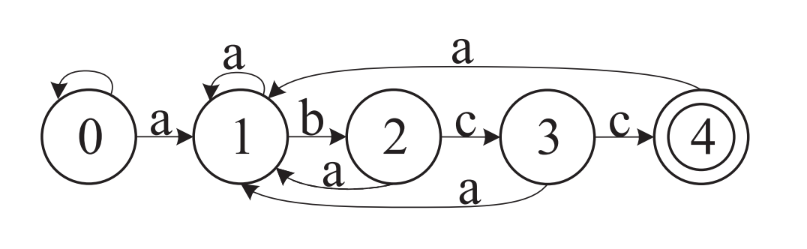
\includegraphics[width=0.5\textwidth]{fig2}
    \caption{通过字符串abcc构建的DFA}
    \label{fig:fig2}
\end{figure}

\begin{figure}[h]
    \centering
    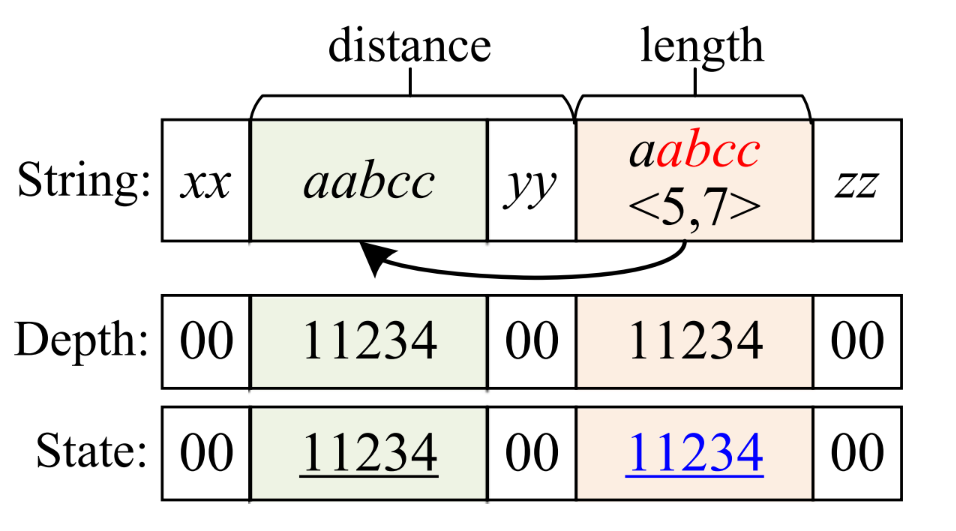
\includegraphics[width=0.5\textwidth]{fig3}
    \caption{要处理的压缩数据,第二个aabcc用<5,7>表示,5表示字符串长度,7表示与第一个aabcc的距离。}
    \label{fig:fig3}
\end{figure}

\vspace{3mm}
\subsection{数据来源}
数据来源有以下两个:
\begin{enumerate}
  \item Alexa.com和Alexa.cn前500名的网站页面流量
  \item 校园网网关出口收集到的流量
\end{enumerate}

\vspace{3mm}
\subsection{测试方案}
测试方案选取Alexa.com和Alexa.cn前500名的网站以及校园网网关收集数据作为原始流量数据,选取不同数量的Snort规则(snort24,snort31,snort34,snort135)作为要匹配的模式,在相同数据集下测试实现的高性能算法,主要包含三组对比测试:
\begin{enumerate}
  \item 与非压缩流量算法性能对比
  \item 与hyperscan算法性能对比
  \item 校园网网关出口真实流量测试
\end{enumerate}

\vspace{8mm}
\section{进度安排,预期达到的目标}

\begin{table}[h]
\begin{tabular}{|l|l|}
\hline
2021.11-2021.12 & \begin{tabular}[c]{@{}l@{}}查询各种压缩流量下的字符串匹配算法的原论文并进行实现,\\ 在测试数据下测试其正确性\end{tabular}           \\ \hline
2022.1-2022.2   & \begin{tabular}[c]{@{}l@{}}对实现的程序在收集到的压缩数据下进行测试,\\ 比较运行效率和占用内存\end{tabular}                  \\ \hline
2022.3          & \begin{tabular}[c]{@{}l@{}}根据比较的结果,改进算法,实现压缩流量场景下的高性能算法,\\ 并在收集的流量数据下与原匹配算法进行比较\end{tabular} \\ \hline
2022.4          & 根据最终结果,完成毕业论文                                                                                \\ \hline
\end{tabular}
\end{table}

\vspace{8mm}
\section{课题已具备和所需的条件、经费}
系统平台:Linux

硬件环境:
\begin{itemize}
  \item CPU:Intel i5-8265U (8) @ 3.900GHz
  \item GPU:NVIDIA GeForce MX250    
  \item 内存:8GB
  \item 硬盘容量:512GB
\end{itemize}

编程语言:C++

软件环境:Visual Studio Code

\vspace{8mm}
\section{研究过程中可能遇到的困难和问题,解决的措施}
\begin{enumerate}
  \item 算法改进:\\对字符串匹配算法的优化、压缩没有太深的了解。在实现字符串匹配算法的同时进一步学习,同时查阅各算法的原论文,掌握其思想。
  \item 数据处理:\\Snort规则基于正则表达式,因此需要首先转化为DFA才能进行匹配。许多库函数实现了正则表达式转化为DFA,可以直接调用或者自己根据正则表达式转化为DFA的方法\cite{张树壮2011面向网络安全的正则表达式匹配技术}实现。
  \item 编程实现:\\本课题计划通过C++实现算法,CMake作为组建自动化工具,目前来讲对于整体的程序设计和程序测试上缺乏经验,需要一段时间去熟悉。
\end{enumerate}

\vspace{8mm}
\section{主要参考文献}

\bibliographystyle{hithesis}
\bibliography{references}
